% Iteration 2 chapter for the EquiFlow FYP report.
% Put this file in chapters/, results_tables.tex next to it, and docs/figures/*.pdf in figures/.
% In main.tex: \input{chapters/chapter7_iteration2} after chapter6_iteration1.
% Needs \usepackage{graphicx} (loaded by most report classes).
% All numbers come from sumo/results/heldout/*.csv (see docs/RESULTS.md); the tables are generated by
% sumo/latex_tables.py and should be regenerated rather than edited.

\chapter{Iteration 2: Tracking, Control, Integration and Evaluation}
\label{ch:iteration2}

\section{Iteration Objectives}
Iteration~2 turns the perception and simulation work of Iteration~1 into a working, measured system.
Its objectives, taken from the iteration plan, were to:
(i) track ambulances across frames so that a single confident frame cannot trigger priority;
(ii) give a confirmed ambulance a protected green through safe yellow and all-red transitions, also across
neighbouring junctions (green corridor);
(iii) restore service to delayed approaches afterwards (fair recovery) and add a fairness-aware MARL base
controller;
(iv) integrate the modules behind FastAPI and MQTT with a live dashboard; and
(v) evaluate the controllers on repeatable SUMO runs against fixed-time and actuated baselines.
The exit criterion was that a scripted ambulance scenario triggers and completes a logged preemption with
recovery.

\section{Selected Use Cases / Features}
UC-01 (detect an approaching ambulance), UC-02 (estimate traffic state), UC-03 (grant emergency priority),
UC-04 (recover fairly after priority), UC-05 (run a baseline comparison) and UC-06 (monitor the junction on
the dashboard). Requirement coverage after this iteration is summarised in Table~\ref{tab:it2-req}.

\begin{table}[htbp]
\centering
\small
\caption{Functional requirements and test cases addressed in Iteration 2.}
\label{tab:it2-req}
\resizebox{\textwidth}{!}{%
\begin{tabular}{lll}
\hline
Requirement / test & Implementation & Evidence \\
\hline
FR-01--03 detection input, output, logging & \texttt{vision/live.py}, \texttt{eventlog.py} & \texttt{test\_live\_pipeline.py}, CSV event log \\
FR-04 traffic state & SUMO queues; camera approach zones (\texttt{zones:}) & \texttt{test\_fr04\_zone\_...} \\
FR-05 / TC-03 stale detections & 2\,s age limit on external events, K-of-M vote, 60\,s fail-safe & \texttt{test\_tc03\_...} \\
FR-06--08 phases, timing, priority & \texttt{controllers/intersection.py} & \texttt{test\_controller.py} (randomised safety) \\
FR-07 / TC-04 early end of empty green & gap-out after 5\,s, only if another approach has demand & \texttt{test\_tc04\_...} \\
FR-09 / TC-06 logged preemption and recovery & event log + episode table & \texttt{scripts/scripted\_scenario.py} \\
FR-10 recovery uses queue and wait & queue-sized recovery greens, longest wait first & \texttt{test\_fr10\_...} \\
FR-11 baselines & fixed-time, actuated, fixed-time + priority & Section~\ref{sec:it2-results} \\
FR-12 export metrics and configuration & \texttt{run\_manifest.csv} (config + versions per run) & \texttt{results/heldout/} \\
TC-10 repeatability & same seed and configuration give identical results & \texttt{test\_tc10\_...} \\
\hline
\end{tabular}}
\end{table}

\section{Design}
The controller is split into a \emph{base controller} that chooses the next green in normal operation
(fixed-time, adaptive, or the MARL policy) and an \emph{intersection controller} that wraps it with
everything that must never be learned: ambulance priority, minimum green, yellow and all-red, the 90\,s
maximum-wait guard, gap-out and fair recovery. The intersection controller never reads a clock; it is
given the time on every tick, so the same code runs in the live backend (every 0.1\,s) and inside each SUMO
step. Every decision is published as an event on a bus that feeds the REST/WebSocket API, the optional MQTT
bridge and a CSV event log.

\section{Implementation}
\begin{itemize}
\item \textbf{Perception} (\texttt{backend/app/vision/live.py}): YOLO26s vehicle detection with ByteTrack,
the cls\_v4 classifier on each tracked crop, and a confirmation vote (5 of the last 8 frames, mean score at
least 0.65). Optional per-approach polygons restrict counting to the lanes that queue for the signal and
report stationary vehicles as the queue.
\item \textbf{Signal control} (\texttt{backend/app/controllers/}): base controllers, the MARL policy
(shared Q-network over per-phase features, pure NumPy) and the intersection controller described above.
\item \textbf{Integration} (\texttt{backend/app/}): FastAPI REST + WebSocket + MJPEG, MQTT topics, a live
SUMO view driven through TraCI, an optional API key on every write endpoint, and the CSV event log.
\item \textbf{Evaluation} (\texttt{sumo/}): \texttt{run\_matrix.py} runs every controller on the same
networks, demand levels and seeds in parallel; \texttt{aggregate.py} computes means, confidence intervals and
paired differences; \texttt{make\_plots.py} and \texttt{latex\_tables.py} produce the figures and tables in
this chapter.
\end{itemize}

\section{Algorithms and Technical Decisions}
\paragraph{Gap-out.} A green that has run at least 5\,s ends early when no vehicle is within 120\,m of its
stop line and another approach has demand. It is never applied during priority and always passes through
the full yellow and all-red.
\paragraph{Priority.} After the vote confirms an ambulance, the current green finishes its minimum time,
then yellow and all-red, and the ambulance's approach turns green alone. Priority ends 4\,s after the
ambulance was last seen, or after 60\,s as a fail-safe. Two ambulances are served first come, first served.
\paragraph{Fair recovery.} After priority, the approaches that were held red and have a queue are served in
order of longest wait, each for about as long as its queue needs to clear (2\,s per queued vehicle, at least
5\,s, at most 30\,s). A first version gave every delayed approach a fixed 15\,s green plus extra; it was
replaced after the ablation in Section~\ref{sec:it2-ablation} showed it lengthened the longest waits.
\paragraph{Stale detections.} An externally reported detection older than 2\,s (or more than 2\,s in the
future) is rejected and logged, so a delayed or replayed message cannot request priority.

\section{Evaluation Set-up}
Six signalised Islamabad junction networks were each run at four demand levels for one simulated hour.
Every controller used the same 120 network/demand/seed combinations with seeds 6--10; the MARL policy was
trained on seeds 1--5, so all evaluation runs are held out. Ambulances are confirmed by a virtual camera per
approach using the real voting rule. Results are reported as mean $\pm$ 95\% confidence interval over runs,
and as \emph{paired} differences on identical runs, which removes the large differences between networks.

% Generated by sumo/latex_tables.py from the CSV results. Do not edit by hand; re-run the script.

\begin{table}[htbp]
\centering
\small
\caption{Held-out evaluation: mean $\pm$ 95\% confidence interval over one-hour SUMO runs (seeds 6--10).}
\label{tab:it2-main}
\resizebox{\textwidth}{!}{%
\begin{tabular}{lccccc}
\hline
Metric & Fixed-time & Actuated & Fixed + priority & EquiFlow & EquiFlow (MARL) \\
\hline
Car mean wait (s) & 16.87 $\pm$ 1.02 & 6.28 $\pm$ 1.01 & 10.38 $\pm$ 0.86 & 5.38 $\pm$ 0.44 & 5.39 $\pm$ 0.54 \\
Ordinary vehicles, mean wait (s) & 17.07 $\pm$ 1.05 & 6.23 $\pm$ 0.99 & 10.30 $\pm$ 0.84 & 5.36 $\pm$ 0.43 & 5.34 $\pm$ 0.54 \\
95th-percentile wait (s) & 51.71 $\pm$ 1.61 & 17.87 $\pm$ 2.13 & 29.55 $\pm$ 1.69 & 18.45 $\pm$ 1.18 & 20.31 $\pm$ 1.58 \\
Longest single wait (s) & 72.17 $\pm$ 3.72 & 36.71 $\pm$ 4.45 & 58.98 $\pm$ 5.08 & 39.44 $\pm$ 3.11 & 42.67 $\pm$ 3.50 \\
Share waiting $>$60 s & 0.030 $\pm$ 0.005 & 0.002 $\pm$ 0.001 & 0.003 $\pm$ 0.001 & 0.000 $\pm$ 0.000 & 0.001 $\pm$ 0.001 \\
Worst approach, mean wait (s) & 21.98 $\pm$ 1.37 & 7.95 $\pm$ 1.10 & 13.49 $\pm$ 1.02 & 6.92 $\pm$ 0.52 & 6.97 $\pm$ 0.61 \\
Jain index across approaches & 0.915 $\pm$ 0.025 & 0.888 $\pm$ 0.025 & 0.903 $\pm$ 0.025 & 0.909 $\pm$ 0.024 & 0.895 $\pm$ 0.027 \\
Ambulance mean wait (s) & 13.75 $\pm$ 1.16 & 7.42 $\pm$ 1.31 & 0.19 $\pm$ 0.08 & 0.10 $\pm$ 0.06 & 0.07 $\pm$ 0.04 \\
Ambulance travel time (s) & 59.14 $\pm$ 2.42 & 52.75 $\pm$ 2.40 & 43.11 $\pm$ 2.19 & 42.68 $\pm$ 2.20 & 42.72 $\pm$ 2.21 \\
Detection to green (s) & -- & -- & 2.58 $\pm$ 0.16 & 2.41 $\pm$ 0.12 & 2.51 $\pm$ 0.14 \\
Recovery interval (s) & -- & -- & 0.00 $\pm$ 0.00 & 22.99 $\pm$ 0.96 & 22.70 $\pm$ 0.92 \\
Runs & 120 & 120 & 120 & 120 & 120 \\
\hline
\end{tabular}}
\end{table}

\begin{table}[htbp]
\centering
\small
\caption{Ablations: EquiFlow with one component switched off (the corridor ablation runs only on the two multi-junction networks).}
\label{tab:it2-ablation}
\resizebox{\textwidth}{!}{%
\begin{tabular}{lccccc}
\hline
Metric & EquiFlow & Old recovery rule & No recovery & No gap-out & No corridor \\
\hline
Car mean wait (s) & 5.38 $\pm$ 0.44 & 5.48 $\pm$ 0.47 & 5.35 $\pm$ 0.42 & 6.57 $\pm$ 0.54 & 4.80 $\pm$ 0.42 \\
95th-percentile wait (s) & 18.45 $\pm$ 1.18 & 19.08 $\pm$ 1.35 & 18.37 $\pm$ 1.16 & 20.68 $\pm$ 1.38 & 16.09 $\pm$ 0.91 \\
Longest single wait (s) & 39.44 $\pm$ 3.11 & 41.72 $\pm$ 3.41 & 38.83 $\pm$ 3.09 & 42.54 $\pm$ 3.34 & 32.00 $\pm$ 2.42 \\
Jain index across approaches & 0.909 $\pm$ 0.024 & 0.910 $\pm$ 0.025 & 0.910 $\pm$ 0.025 & 0.907 $\pm$ 0.024 & 0.774 $\pm$ 0.053 \\
Ambulance mean wait (s) & 0.10 $\pm$ 0.06 & 0.11 $\pm$ 0.05 & 0.12 $\pm$ 0.07 & 0.12 $\pm$ 0.06 & 0.02 $\pm$ 0.02 \\
Ambulance travel time (s) & 42.68 $\pm$ 2.20 & 42.75 $\pm$ 2.19 & 42.73 $\pm$ 2.20 & 42.85 $\pm$ 2.20 & 55.14 $\pm$ 4.60 \\
Recovery interval (s) & 22.99 $\pm$ 0.96 & 28.09 $\pm$ 1.37 & 0.00 $\pm$ 0.00 & 27.05 $\pm$ 1.12 & 20.43 $\pm$ 0.48 \\
Runs & 120 & 120 & 120 & 120 & 40 \\
\hline
\end{tabular}}
\end{table}

\begin{table}[htbp]
\centering
\small
\caption{Paired comparison on identical runs (same network, demand and seed): EquiFlow minus the other controller. Negative values mean EquiFlow is lower. $^*$: the 95\% CI excludes zero.}
\label{tab:it2-paired}
\begin{tabular}{llccc}
\hline
Versus & Metric & Difference (95\% CI) & EquiFlow better in & Runs \\
\hline
Fixed-time & Car mean wait (s) & -11.49 $\pm$ 0.68$^*$ & 100\% & 120 \\
Fixed-time & 95th-percentile wait (s) & -33.26 $\pm$ 1.01$^*$ & 100\% & 120 \\
Fixed-time & Longest single wait (s) & -32.73 $\pm$ 3.28$^*$ & 98\% & 120 \\
Fixed-time & Ambulance mean wait (s) & -13.64 $\pm$ 1.13$^*$ & 100\% & 120 \\
Actuated & Car mean wait (s) & -0.90 $\pm$ 0.74$^*$ & 38\% & 120 \\
Actuated & 95th-percentile wait (s) & +0.58 $\pm$ 1.34 & 31\% & 120 \\
Actuated & Longest single wait (s) & +2.73 $\pm$ 3.33 & 32\% & 120 \\
Actuated & Ambulance mean wait (s) & -7.32 $\pm$ 1.30$^*$ & 99\% & 120 \\
Fixed + priority & Car mean wait (s) & -5.00 $\pm$ 0.49$^*$ & 100\% & 120 \\
Fixed + priority & 95th-percentile wait (s) & -11.09 $\pm$ 0.74$^*$ & 100\% & 120 \\
Fixed + priority & Longest single wait (s) & -19.53 $\pm$ 2.96$^*$ & 92\% & 120 \\
Fixed + priority & Ambulance mean wait (s) & -0.09 $\pm$ 0.08$^*$ & 28\% & 120 \\
EquiFlow (MARL) & Car mean wait (s) & -0.00 $\pm$ 0.17 & 43\% & 120 \\
EquiFlow (MARL) & 95th-percentile wait (s) & -1.85 $\pm$ 0.56$^*$ & 53\% & 120 \\
EquiFlow (MARL) & Longest single wait (s) & -3.23 $\pm$ 2.00$^*$ & 58\% & 120 \\
EquiFlow (MARL) & Ambulance mean wait (s) & +0.03 $\pm$ 0.04 & 10\% & 120 \\
No recovery & Car mean wait (s) & +0.03 $\pm$ 0.09 & 48\% & 120 \\
No recovery & 95th-percentile wait (s) & +0.08 $\pm$ 0.23 & 30\% & 120 \\
No recovery & Longest single wait (s) & +0.61 $\pm$ 1.58 & 35\% & 120 \\
No recovery & Ambulance mean wait (s) & -0.02 $\pm$ 0.06 & 12\% & 120 \\
No gap-out & Car mean wait (s) & -1.18 $\pm$ 0.16$^*$ & 97\% & 120 \\
No gap-out & 95th-percentile wait (s) & -2.22 $\pm$ 0.34$^*$ & 84\% & 120 \\
No gap-out & Longest single wait (s) & -3.10 $\pm$ 1.70$^*$ & 62\% & 120 \\
No gap-out & Ambulance mean wait (s) & -0.02 $\pm$ 0.04 & 20\% & 120 \\
Old recovery rule & Car mean wait (s) & -0.10 $\pm$ 0.09$^*$ & 53\% & 120 \\
Old recovery rule & 95th-percentile wait (s) & -0.62 $\pm$ 0.31$^*$ & 48\% & 120 \\
Old recovery rule & Longest single wait (s) & -2.27 $\pm$ 1.73$^*$ & 56\% & 120 \\
Old recovery rule & Ambulance mean wait (s) & -0.01 $\pm$ 0.05 & 15\% & 120 \\
\hline
\end{tabular}
\end{table}

\begin{table}[htbp]
\centering
\small
\caption{MARL minus adaptive EquiFlow on identical runs, split by whether the network/demand combination was used in MARL training. All seeds are unseen. Negative = MARL lower.}
\label{tab:it2-marl}
\begin{tabular}{lcc}
\hline
Metric & Trained combinations & Unseen combinations \\
\hline
Car mean wait (s) & +0.13 $\pm$ 0.30 (n=40) & -0.06 $\pm$ 0.22 (n=80) \\
95th-percentile wait (s) & +1.77 $\pm$ 0.93 (n=40) & +1.89 $\pm$ 0.71 (n=80) \\
Jain index across approaches & -0.008 $\pm$ 0.007 (n=40) & -0.017 $\pm$ 0.008 (n=80) \\
Ambulance mean wait (s) & -0.03 $\pm$ 0.02 (n=40) & -0.03 $\pm$ 0.07 (n=80) \\
\hline
\end{tabular}
\end{table}

\begin{table}[htbp]
\centering
\small
\caption{Signal controller timing on one CPU core (sumo/benchmark.py). The live backend ticks every 100\,000\,$\mu$s.}
\label{tab:it2-perf}
\begin{tabular}{lcccc}
\hline
Measured & Mean ($\mu$s) & Median & p99 & Max \\
\hline
tick (fixed\_time) & 0.94 & 0.92 & 3.21 & 99.37 \\
decision (fixed\_time) & 0.42 & 0.38 & 0.63 & 467.97 \\
tick (adaptive) & 1.07 & 0.95 & 3.77 & 680.95 \\
decision (adaptive) & 1.39 & 1.2 & 2.68 & 935.52 \\
tick (marl) & 1.35 & 0.94 & 5.07 & 173.0 \\
decision (marl) & 23.83 & 19.82 & 61.69 & 4408.28 \\
\hline
\end{tabular}
\end{table}

\begin{table}[htbp]
\centering
\small
\caption{Tracking pipeline (YOLO26s + ByteTrack + classifier, 5-of-8 vote) on the Islamabad videos. A pass counts as detected if confirmed within 1\,s of its hand-labelled window.}
\label{tab:it2-tracking}
\begin{tabular}{lcccccc}
\hline
Video & Crops used in & Passes & Detected & Missed & False events & Latency (s) \\
\hline
test1 & no & 1 & 1 & 0 & 0 & 0.20 \\
test12 & no & 3 & 2 & 1 & 0 & 0.00 0.68 \\
test2 & no & 1 & 1 & 0 & 0 & 0.13 \\
test3 & no & 1 & 1 & 0 & 0 & 0.43 \\
test4 & no & 1 & 1 & 0 & 1 & 0.13 \\
test5 & no & 0 & 0 & 0 & 9 & -- \\
test9 & val & 0 & 0 & 0 & 1 & -- \\
v1 & train & 0 & 0 & 0 & 2 & -- \\
\hline
\end{tabular}
\end{table}



\section{Results}
\label{sec:it2-results}
\begin{figure}[htbp]
\centering
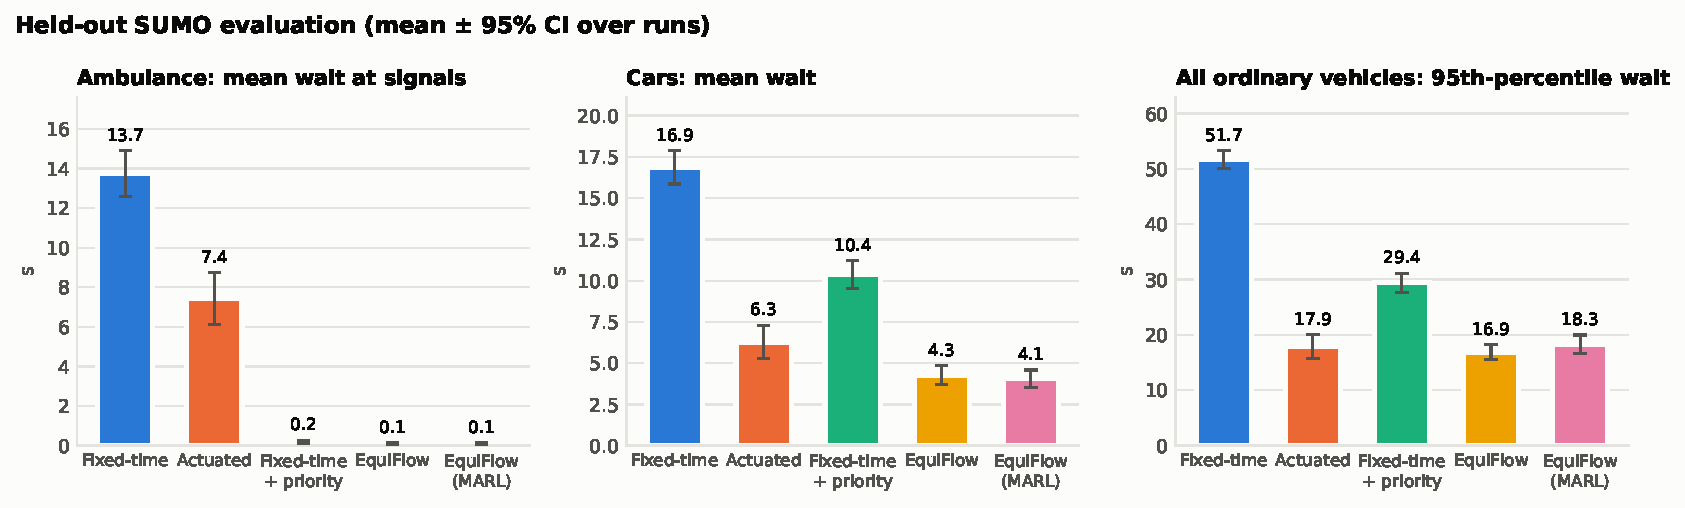
\includegraphics[width=\textwidth]{figures/fig_main_comparison.pdf}
\caption{Held-out evaluation: ambulance wait, car wait and 95th-percentile wait per controller
(mean $\pm$ 95\% CI over 120 runs each).}
\label{fig:it2-main}
\end{figure}

Table~\ref{tab:it2-main} and Figure~\ref{fig:it2-main} give the main comparison. EquiFlow reduces the
ambulance's mean wait at signals from 13.75\,s (fixed-time) and 7.42\,s (actuated) to 0.10\,s, and its travel
time by 16.5\,s and 10.1\,s respectively. Ordinary traffic does not pay for this on average: car wait is
5.38\,s against 16.87\,s for fixed-time and 6.28\,s for actuated. The paired comparison
(Table~\ref{tab:it2-paired}) shows the advantage over actuated is statistically significant but small
($-0.90 \pm 0.74$\,s) and comes from a minority of runs: EquiFlow is better in 38\% of paired runs. Its
95th-percentile and longest waits are statistically indistinguishable from actuated, and its Jain fairness
index across approaches is significantly higher ($+0.021$, better in 73\% of runs).

\begin{figure}[htbp]
\centering
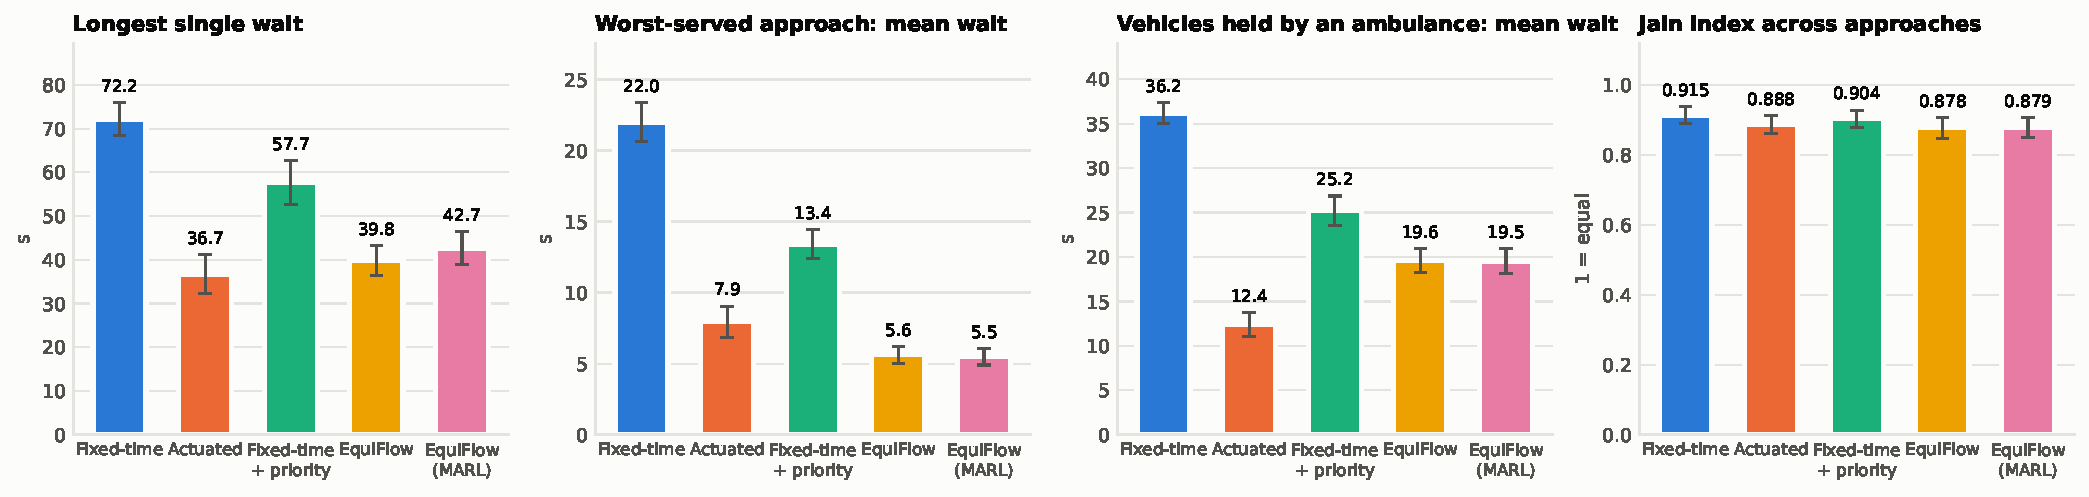
\includegraphics[width=\textwidth]{figures/fig_fairness.pdf}
\caption{Fairness: longest single wait, the worst-served approach's mean wait, and Jain's index across
approaches.}
\label{fig:it2-fairness}
\end{figure}

\begin{figure}[htbp]
\centering
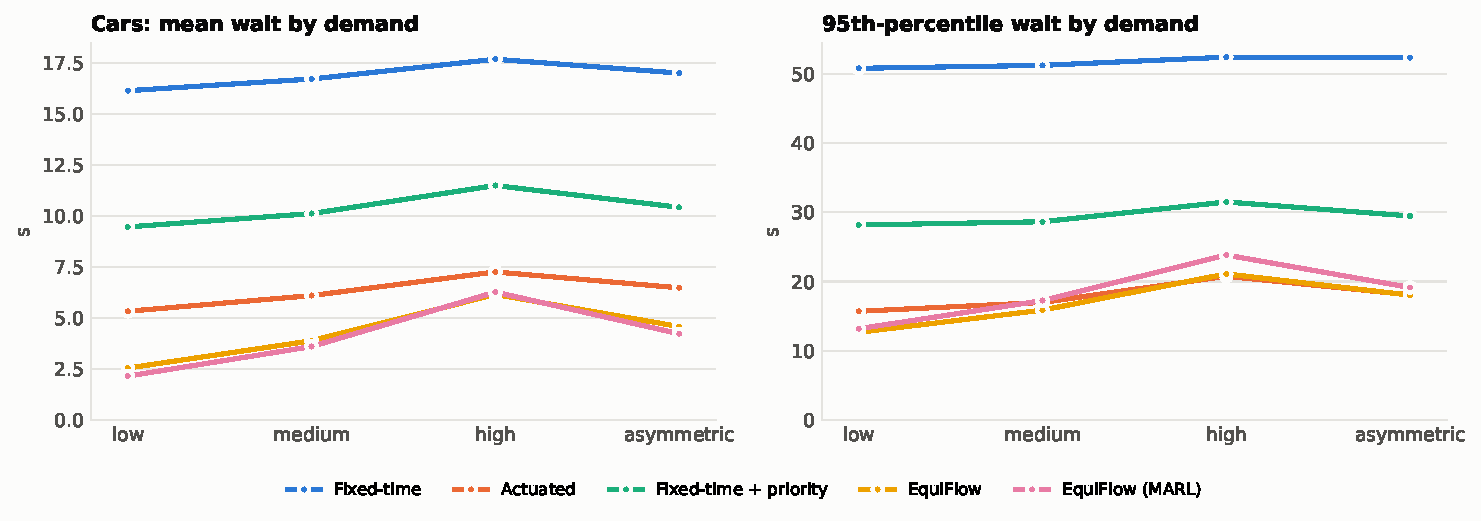
\includegraphics[width=\textwidth]{figures/fig_by_demand.pdf}
\caption{Car mean wait and 95th-percentile wait by demand level.}
\label{fig:it2-demand}
\end{figure}

Under heavy demand (Figure~\ref{fig:it2-demand}) the advantage over actuated shrinks (6.92 against
7.25\,s) and EquiFlow's 95th-percentile wait is higher (22.44 against 20.76\,s): actuated control extends a
green vehicle by vehicle, while the adaptive controller fixes each green's length when it starts.

\subsection{Ablations}
\label{sec:it2-ablation}
\begin{figure}[htbp]
\centering
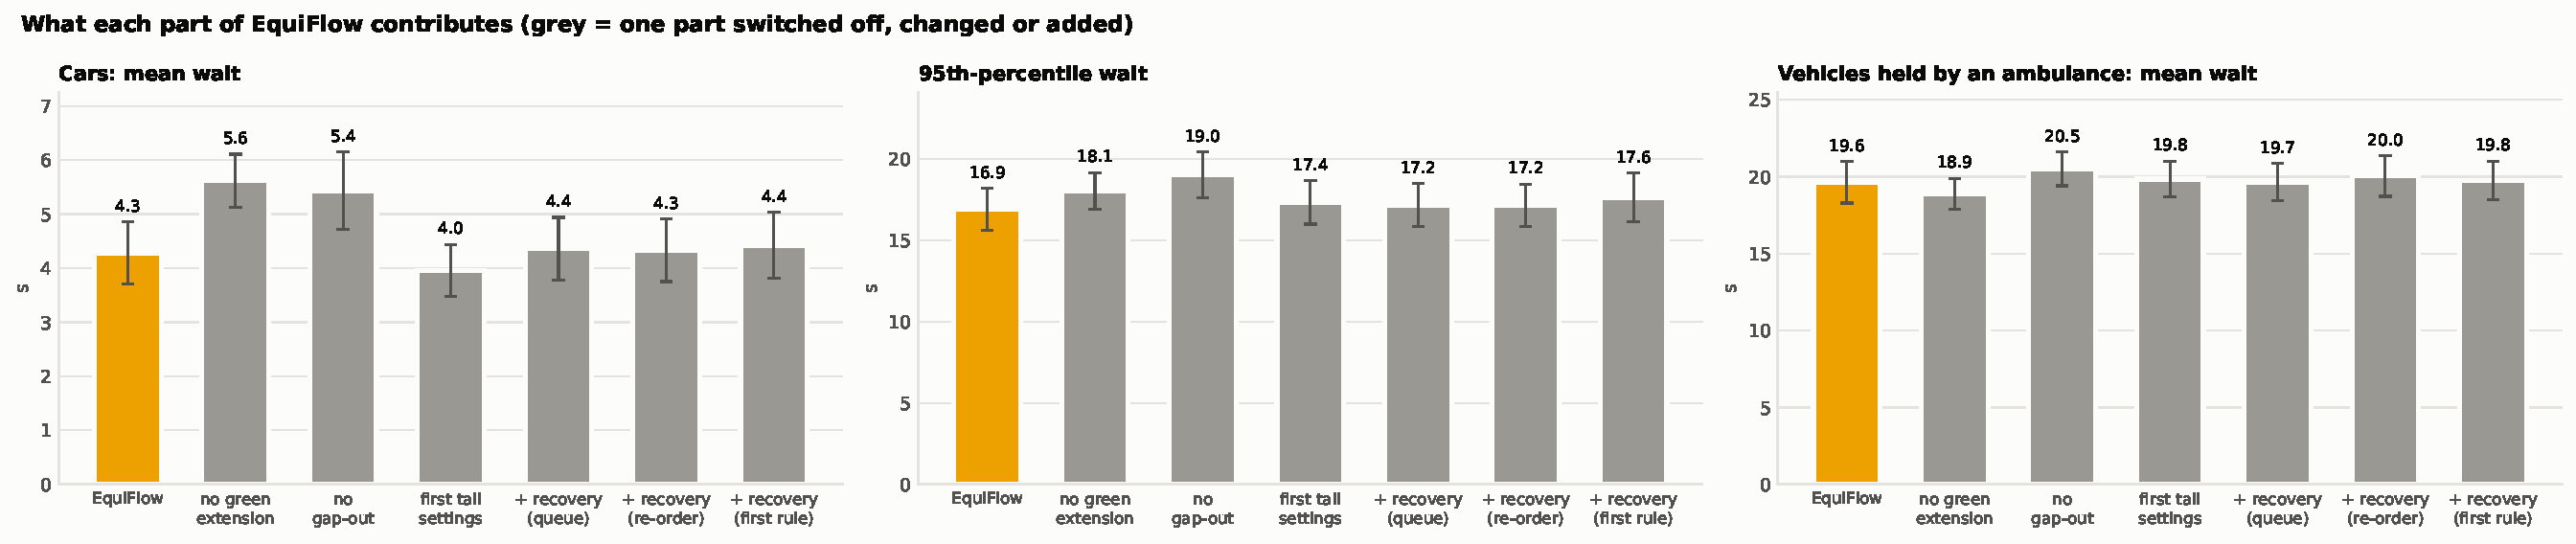
\includegraphics[width=\textwidth]{figures/fig_ablation.pdf}
\caption{Ablations: EquiFlow with one component switched off or replaced.}
\label{fig:it2-ablation}
\end{figure}

Table~\ref{tab:it2-ablation} and Figure~\ref{fig:it2-ablation} switch one component off at a time.
\emph{Gap-out} is the largest single benefit: without it car wait rises by 1.18\,s and the 95th-percentile
wait by 2.22\,s (better in 97\% of paired runs). \emph{Fair recovery} has no measurable effect: with it
switched off, no metric changes significantly. The first recovery rule was slightly harmful (longest wait
2.3\,s worse than the current rule). We attribute this to short priority intervals (about 12--15\,s), an
adaptive base controller that already serves the longest-waiting busy approach, the 90\,s maximum-wait guard,
and network-wide metrics that dilute an effect confined to the vehicles caught by a priority interval.
The \emph{green corridor} (evaluated on the two multi-junction networks) makes ambulances 0.21\,s faster but
raises the longest wait of ordinary vehicles by 8.2\,s.

\subsection{MARL controller}
\begin{figure}[htbp]
\centering
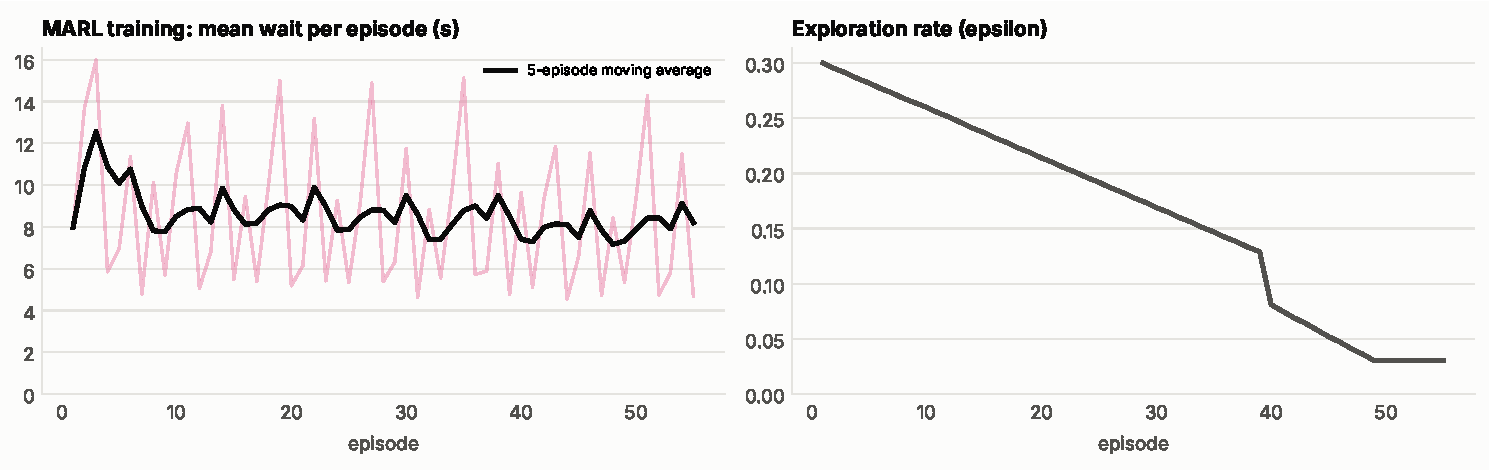
\includegraphics[width=\textwidth]{figures/fig_marl_training.pdf}
\caption{MARL training: mean wait per episode (episodes rotate between networks) and exploration rate.}
\label{fig:it2-marl}
\end{figure}

On held-out seeds the MARL base controller ties the adaptive heuristic on car wait ($-0.00 \pm 0.17$\,s) and
ambulance wait, but has a higher 95th-percentile wait (+1.85\,s) and a lower Jain index
(Table~\ref{tab:it2-marl}). The gap is the same on network/demand combinations it was trained on and on
unseen ones, so the policy is not over-fitted; it has not yet learned to beat the heuristic after 55 short
training episodes.

\subsection{Robustness to camera errors}
\begin{figure}[htbp]
\centering
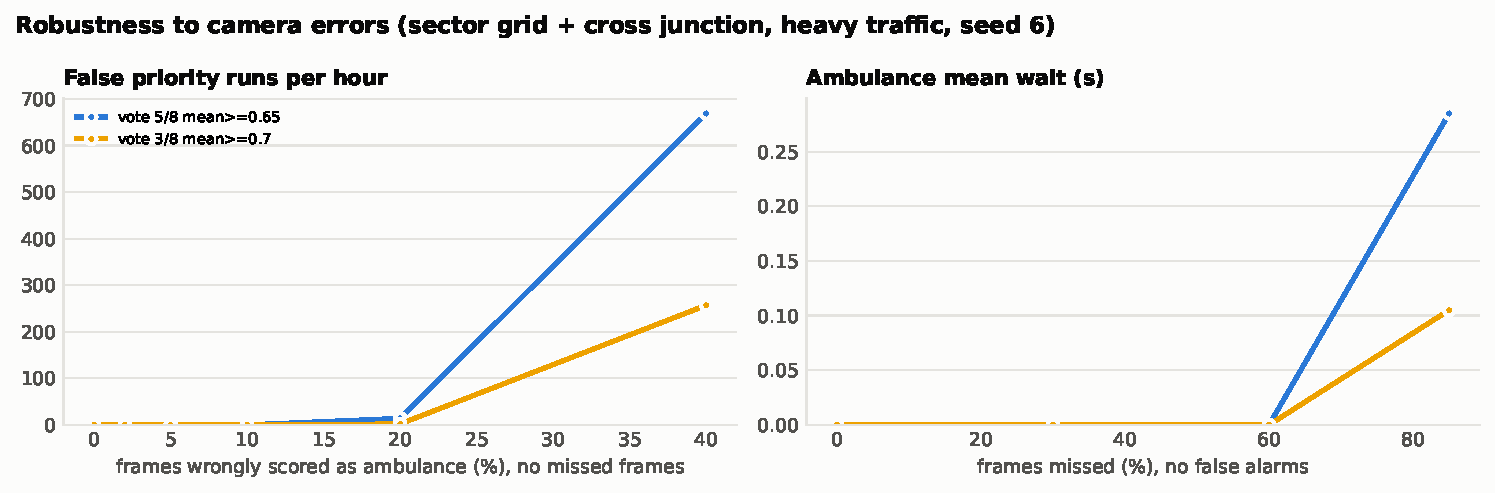
\includegraphics[width=\textwidth]{figures/fig_robustness.pdf}
\caption{False priority runs and ambulance wait as the virtual camera misses frames or scores ordinary
vehicles as ambulances (heavy demand, seed 6).}
\label{fig:it2-robust}
\end{figure}

With up to 10\% of frames wrongly scored as ambulance, the voting rule produces no false priority at all;
at 20\% it produces 6--33 false priority runs per hour, and at 40\% hundreds (Figure~\ref{fig:it2-robust}).
Missing even 85\% of frames barely matters (ambulance wait at most 1.8\,s). The classifier's validation
false-alarm rate is 0.65\%, well inside this margin.

\subsection{Tracking on real video}
Table~\ref{tab:it2-tracking} scores the tracking pipeline on the Islamabad clips that have been processed:
6 of 7 ambulance passes are confirmed, on average 0.26\,s after the ambulance appears. Thirteen false
confirmations occur, nine of them in one clip (test5); its ground truth will be re-checked, since most of
these tracks move in the same direction like a single vehicle. The sample is too small for a reliable recall
estimate.

\subsection{Performance}
A controller tick takes about 1\,$\mu$s and a MARL decision about 24\,$\mu$s (p99 62\,$\mu$s), against a
100\,000\,$\mu$s tick period (Table~\ref{tab:it2-perf}). A one-hour SUMO run takes about 3\,s.

\section{Failure Analysis}
\begin{table}[htbp]
\centering
\small
\caption{Failure cases found in Iteration 2 and the planned response.}
\label{tab:it2-failures}
\resizebox{\textwidth}{!}{%
\begin{tabular}{lll}
\hline
Failure & Likely cause & Response \\
\hline
Missed ambulance visible only 2\,s (test12) & fewer than 5 confident frames before it leaves & smaller K for short edge tracks \\
9 false confirmations in test5 & look-alike vehicle, or wrong label & re-check label; add hard negatives \\
Classifier recall 91\% (validation) & 96\,px crops; 17.5\% ambulances in train & val-tuned threshold; 128\,px; oversampling \\
False priority at $\geq$20\% per-frame false alarms & vote too permissive for very noisy input & keep per-frame FP $\ll$ 20\% \\
Higher p95 wait than actuated under heavy demand & green length fixed at its start & per-vehicle green extension \\
Corridor raises longest wait by 8\,s & downstream junctions clear too early & shorter corridor horizon \\
No measurable effect of fair recovery & short priority intervals; diluted metrics & approach-level metrics; stress scenarios \\
\hline
\end{tabular}}
\end{table}

\section{Limitations}
All control results are from simulation; the SUMO cameras are virtual (exact ambulance positions with
simulated classifier scores), so the real camera pipeline and the SUMO evaluation share the controller and the
voting rule but not the video. The detector has not yet been evaluated on the held-out test split. Fairness is
measured network-wide. Authentication is off by default and must be enabled for any deployment.

\section{Iteration Outcome}
The exit criterion is met: the scripted scenario (\texttt{scripts/scripted\_scenario.py}) sends one ambulance,
then two simultaneous ambulances; each is confirmed by detection, receives a protected green, and is followed
by recovery greens, and the whole sequence is recorded in the event log. All 40 automated tests pass. The main
open items for FYP-2 are the detector's test-split evaluation, a recovery policy with a measurable fairness
benefit, longer MARL training, and processing the remaining videos.
